% --------------------------------------
% Chapter 19 Solutions
% --------------------------------------


\subsection{19.5 $\bigstar \bigstar$}
Below is a diagrammatic proof that $*(*\mathbf{F})=-\mathbf{F}$. An explanation:
\begin{itemize}
\item[e)] Swopping two indices in the levi-civita tensor picks up a minus sign.
\item[g)] Two indices are swopped, picking up two minus signs.
\item[h)] Using one of the identities in Penroses Fig 12.18.
\item[i)] Using the fact that $\mathbf{F}$ is an antisymmetric tensor.
\end{itemize}
Using this, we have that
\begin{align*}
*(^\pm \mathbf{F})&=\frac{1}{2}*(\mathbf{F}\mp i*\mathbf{F})\\
&=\frac{1}{2}(*\mathbf{F}\mp i**\mathbf{F})\\
&=\frac{1}{2}(*\mathbf{F}\pm i\mathbf{F})\\
&=\frac{i}{2}((-i)*\mathbf{F}\pm \mathbf{F})\\
&=\pm i^\pm \mathbf{F}
\end{align*}
\begin{figure}\label{e}
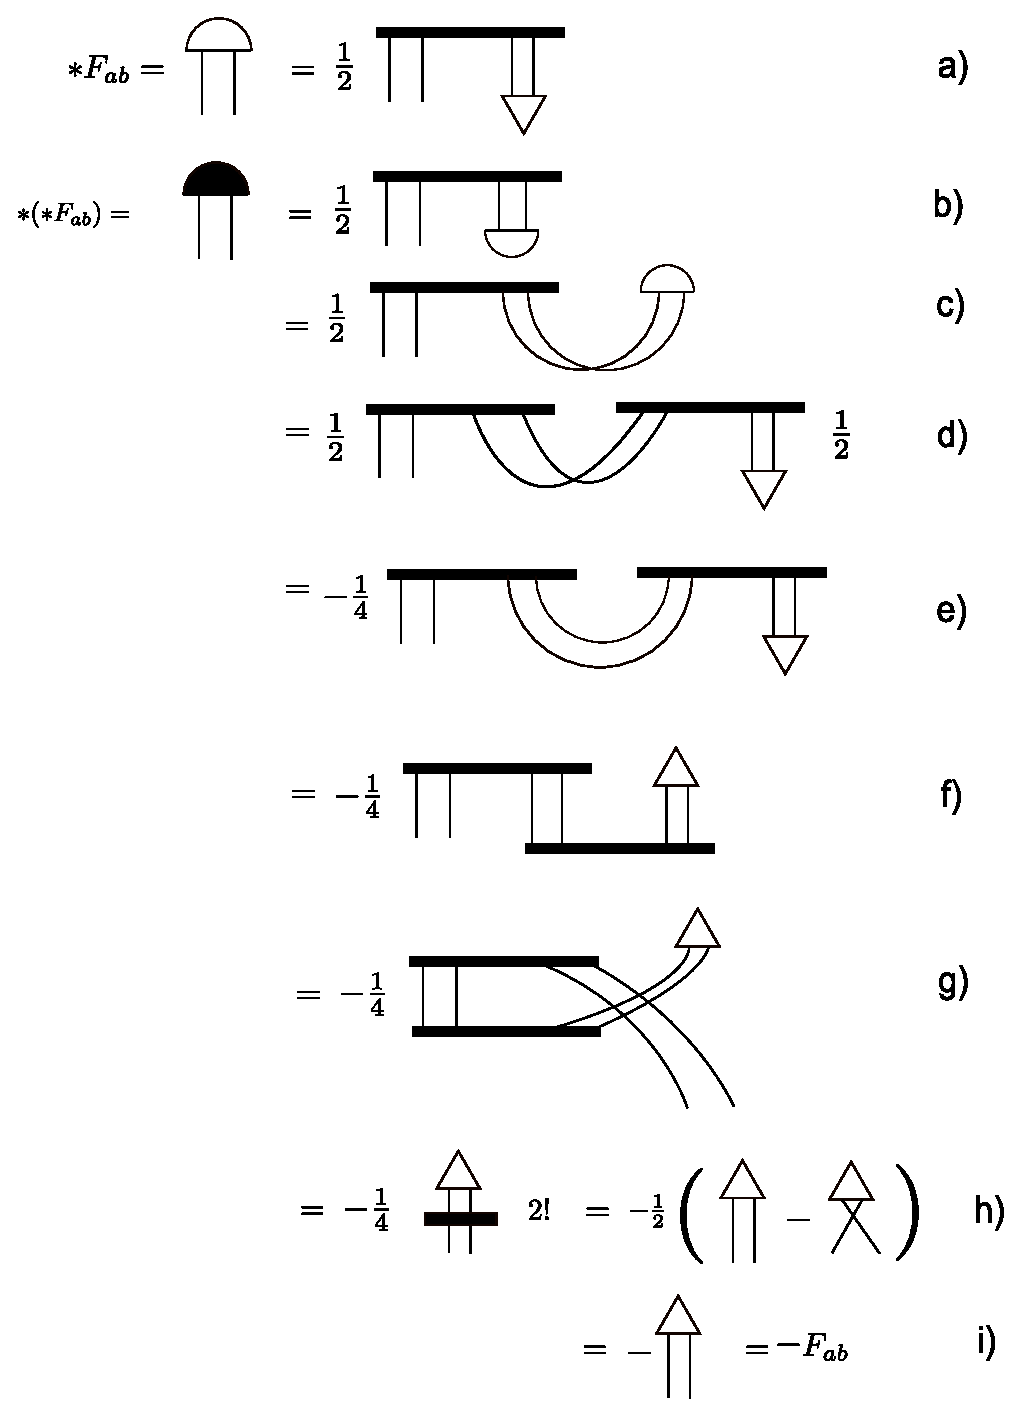
\includegraphics[scale=0.7]{chapters/images/19.5.eps}
\caption{Diagrammatic proof of $*(*\mathbf{F})=-\mathbf{F}$ }
\end{figure} 
